%%%%%%%%%%%%%%%%%%%%%%%%%%%%%%%%%%%%%%%%%%%%%%%%%%%%%%%%%%%%%%%%%%%%
%% I, the copyright holder of this work, release this work into the
%% public domain. This applies worldwide. In some countries this may
%% not be legally possible; if so: I grant anyone the right to use
%% this work for any purpose, without any conditions, unless such
%% conditions are required by law.
%%%%%%%%%%%%%%%%%%%%%%%%%%%%%%%%%%%%%%%%%%%%%%%%%%%%%%%%%%%%%%%%%%%%


\documentclass{beamer}
\usetheme[faculty=fi]{fibeamer}
\usepackage[utf8]{inputenc}
\usepackage[
   main=english, %% By using `czech` or `slovak` as the main locale
                        %% instead of `english`, you can typeset the
                        %% presentation in either Czech or Slovak,
                        %% respectively.
   czech, slovak, greek %% The additional keys allow foreign texts to be
]{babel}            %% typeset as follows:


%% These macros specify information about the presentation
\title{Microbial communities through the lens of high throughput sequencing, data integration and metabolic networks analysis }

\subtitle{on the road to a PhD}
\author{Haris Zafeiropoulos} 

%% These additional packages are used within the document:
\usepackage{ragged2e}                                       % `\justifying` text
\usepackage{booktabs}                                       % Tables
\usepackage{tabularx}
\usepackage{tikz}                                           % Diagrams
\usetikzlibrary{calc, shapes, backgrounds}
\usepackage{amsmath, amssymb}
\usepackage{url}                                            % `\url`s
\usepackage{listings}                                       % Code listings
\usepackage{setspace}
\usepackage[absolute,overlay]{textpos}                      

\frenchspacing

\begin{document}

   \shorthandoff{-}
   \frame[c]{
      \maketitle
   }

   % -------------------------
   %  TOC 
   % -------------------------
   
   % Print an outline at the beginning of sections
   \AtBeginSection[]{
      \begin{frame}<beamer>
         \tableofcontents[currentsection]
      \end{frame}
   }

   % -------------------------
   % CHANGE THE CHAPTER SLIDE 
   % -------------------------
   \begin{darkframes}
      \section{
         Bioinformatics methods for microbial diversity assessment
      }
   
   \end{darkframes}

   % -------------------------
   % CHANGE SUBSECTION: PEMA 
   % -------------------------

   % eDNA SLIDE
   \begin{frame}
      \subsection{\texttt{pema}: a metabarcoding pipeline}
      \frametitle{eDNA metabarcoding}
      \begin{singlespace}


         \begin{columns}[onlytextwidth]

            \column{.5\textwidth}

               \textbf{Marker genes} \\ 

               \begin{enumerate}
                  \item \textbf{16S rRNA:} Bacteria, Archaea
                  \item \textbf{12S rRNA:} Vertebrates
                  \item \textbf{18S rRNA:} Small eukaryotes, Metazoa
                  \item \textbf{ITS:} Fungi
                  \item \textbf{COI:} Eukaryotes
                  \item \textbf{\textit{rbcl}:} Plants
                  \item \textbf{\textit{dsrb}:} Bacteria, Archaea
                  \item ...
               \end{enumerate}

            \column{.45\textwidth}

               \textbf{Bioinformatics analysis steps}

               \begin{enumerate}
                  \item Sequence pre-processing
                  \item OTUs clustering / ASVs inference
                  \item Taxonomic assignment
                  \item Biodiversity analysis
               \end{enumerate}
         
         \end{columns}

      \end{singlespace}
   \end{frame}


   % WORKFLOW SLIDE
   \begin{frame}
      \frametitle{PEMA architecture}
      \begin{singlespace}
         \begin{tikzpicture}[overlay,remember picture]
            \node[anchor=west, xshift=30pt,yshift=-157pt]
               at (current page.north west) {
                  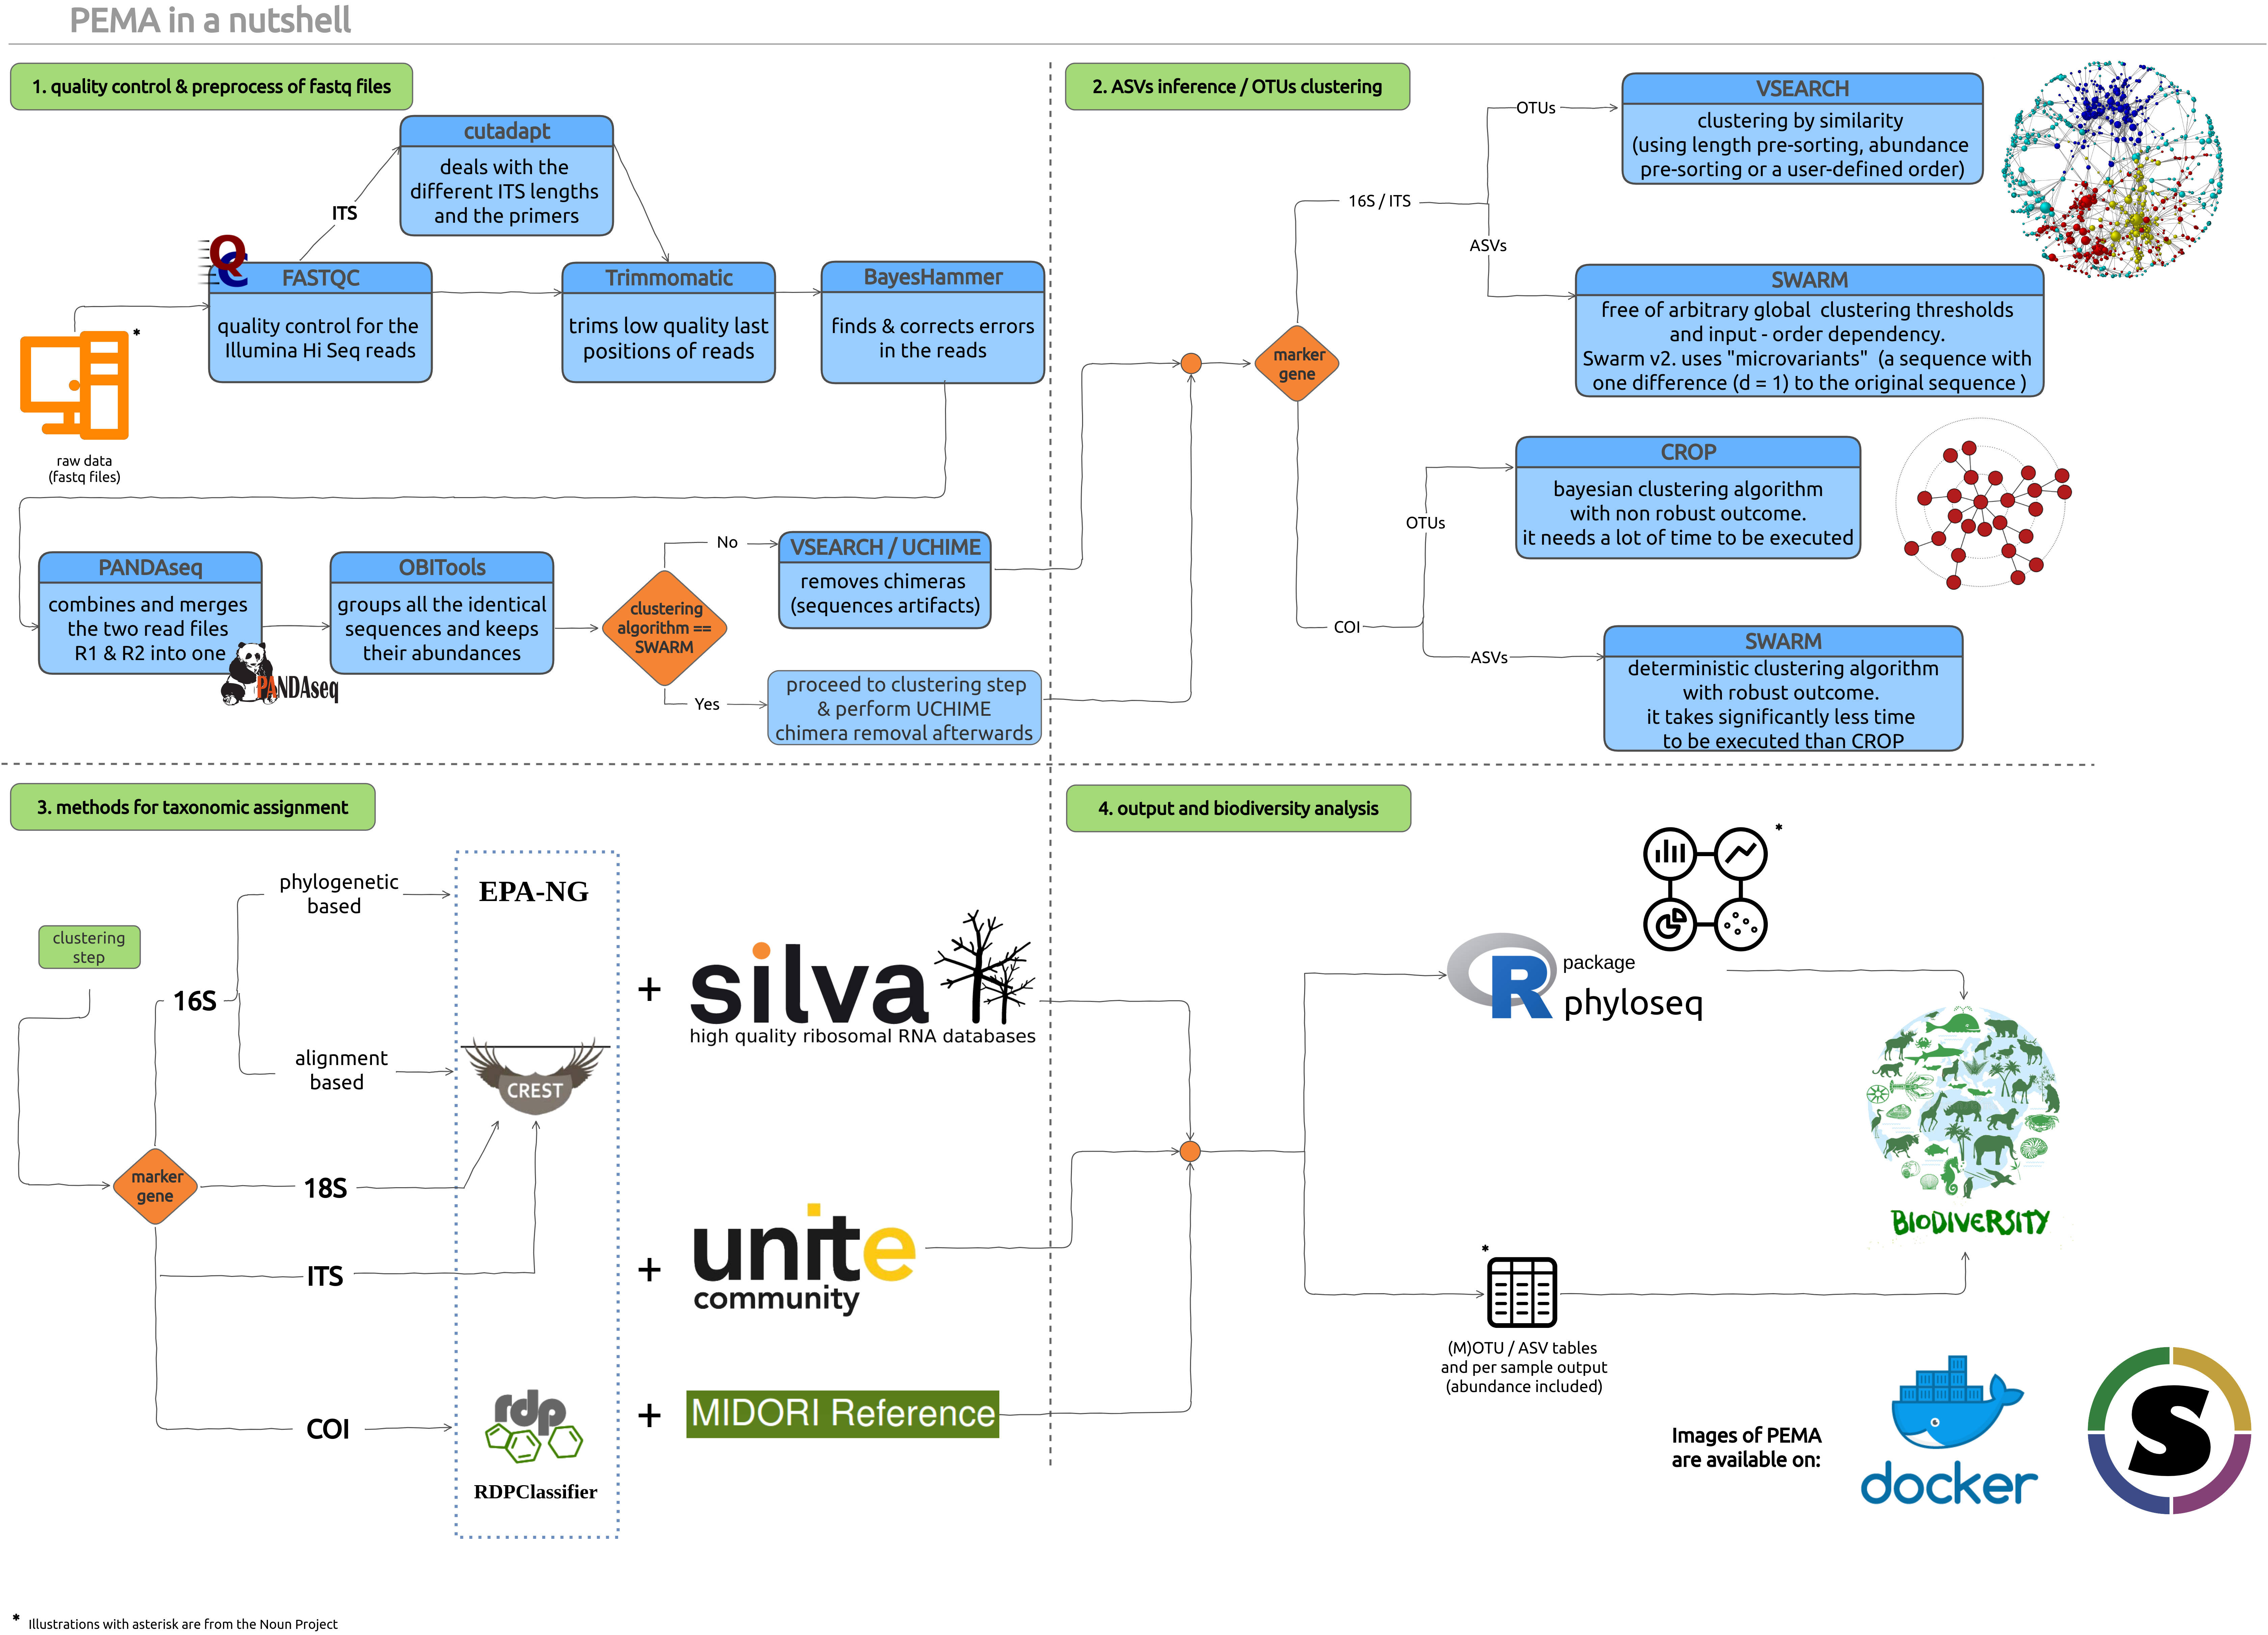
\includegraphics[width=110mm]{resources/pema-pema.drawio.png}
               };

         \end{tikzpicture}
      \end{singlespace}
   \end{frame}

   % BIOINFORMATICS TRICKS AND HINTS
   \begin{frame}
      \frametitle{Being a \texttt{geek} just for a bit !}

      \begin{columns}[onlytextwidth]
         
         \column{0.5\textwidth}
         
            \includegraphics[width=25mm]{resources/bds.png}

            \texttt{BigDataScript} \\
            programming language

         \column{0.5\textwidth}

            \begin{tikzpicture}[overlay,remember picture]

               \node[anchor=east, xshift=-130pt, yshift=10pt]               
                  at (current page.east) {

                     \includegraphics[width=20mm]{resources/sing_transp.png}
                  
                  };

                  \node[anchor=east, xshift=-40pt, yshift=10pt]
                  at (current page.east) {

                     \includegraphics[width=25mm]{resources/docker_facebook_share.png}
                  
                  };

                  \node[anchor=south, align = center, above, xshift=60, yshift=90]
                  at (current page.south) {

                     Containerization

                  };

            \end{tikzpicture}
            
            % \bigskip
            % Containerization


      \end{columns}


   \end{frame}


   % INPUT - OUTPUT - RUN WITH A SINGLE COMMAND
   \begin{frame}

      \frametitle{Mount your I/O}
      \framesubtitle{you give something - you take something}

      \begin{tikzpicture}[overlay,remember picture]

         \node[anchor=west, xshift=10pt, yshift=-10pt]               
            at (current page.west) {

               \includegraphics[width=75mm]{resources/pema_anlysis_dir-Page-1.drawio.png}
            
            };

            \node[anchor=east, xshift=-10pt, yshift=10pt]               
            at (current page.east) {

               \includegraphics[width=35mm]{resources/final_table.jpg}
            
            };

      \end{tikzpicture}
      
   
   \end{frame}



   % PEMA PUBLICATION 
   \begin{frame}
      \frametitle{1st version published in 2020}
      \includegraphics[width=100mm]{resources/pema_publ.png}
   \end{frame}


   % WORKFLOW OF VERSION 2
   \begin{frame}
      \frametitle{PEMA v.2}

      \begin{singlespace}
         \begin{tikzpicture}[overlay,remember picture]
       
               \node[anchor=west, xshift=30pt,yshift=-150pt]
                  at (current page.north west) {
                     \includegraphics[width=110mm]{resources/pema-pema.v2.drawio.png}
                  };
                     
         \end{tikzpicture}
      \end{singlespace}
   \end{frame}


   % PEMA v.2.1.4 - ARMS
   \begin{frame}
      \frametitle{Latest PEMA version}
      \framesubtitle{addressing the challenges of the community}

      \begin{singlespace}
         \begin{tikzpicture}[overlay,remember picture]
       
               \node[anchor=west, xshift=30pt,yshift=-150pt]
                  at (current page.north west) {
                     \includegraphics[width=55mm]{resources/Autonomous-Reef-Monitoring.png}
               };

               \node[anchor=east, xshift=-65pt,yshift=50pt]
                  at (current page.east) {
                     \includegraphics[width=34mm]{resources/assemble_logo.png}
               };

               \node[anchor=east, xshift=-5pt,yshift=50pt]
                  at (current page.east) {
                     \includegraphics[width=17mm]{resources/MBON_logo_transparent.png}

               };

         \end{tikzpicture}


         \begin{textblock*}{5cm}(7.2cm,4.0cm) % {block width} (coords) 
            
            \scriptsize

            \textbf{\texttt{pema:v.2.1.4} includes:}

            \begin{enumerate}
               \item analysis of 12S rRNA data now supported
                     (\href{https://github.com/terrimporter/12SvertebrateClassifier/releases}{12S Vertebrate Classifier v2.0.0-ref} database) 
               \item PR2 as an alternative reference 
                     database for the case of 18S rRNA 
               \item the \texttt{ncbi-taxonomist} tool \\ 
                     was added to return the NCBI Taxonomy \\ 
                     Id of the taxonomies found
            \end{enumerate}

         \end{textblock*}


      \end{singlespace}
   \end{frame}

   % GitHub repo
   \begin{frame}
   \frametitle{open source is cool}
      \framesubtitle{interacting with the community}

      \includegraphics[width=60mm]{resources/pema_contribution.png}

      \small
      \begin{textblock*}{5cm}(7.5cm,4.0cm) % {block width} (coords) 
         PEMA aims at building a community 
         to discuss challenges on metabarcoding
         come up with solutions and why not 
         develop some of them! 
      \end{textblock*}

   \end{frame}



   % PEMA WEBSITE
   \begin{frame}
      \frametitle{\textit{How to} and further documentation}
      \framesubtitle{at \href{http://pema.hcmr.gr}{pema.hcmr.gr}}
      \includegraphics[width=85mm]{resources/pema_site.png}
   \end{frame}




   % -------------------------
   % CHANGE SUBSECTION: DARN
   % -------------------------
   \begin{frame}
      \subsection{\texttt{darn}: known unknowns in COI amplicon data}
      \frametitle{DARN: investigating known \\ unknown in COI amplicon data}
      \begin{singlespace}
         \begin{tikzpicture}[overlay,remember picture]
            \node[anchor=north east, xshift=-10pt,yshift=-5pt]
               at (current page.north east) {
                  \includegraphics[width=50mm]{resources/darn_methodology_transparent.png}
               };
            \node[align = left, above, yshift=10] at (current page.south) {
               \scriptsize 
               Figure from: Heirendt, Laurent, et al. Nature protocols 14.3 (2019): 639-702.
            };
         \end{tikzpicture}
      \end{singlespace}
   \end{frame}





   % -------------------------
   % CHANGE THE CHAPTER SLIDE 
   % -------------------------
   \begin{darkframes}
      \section{
         \texttt{PREGO}: a knowledge-base for organisms - environments - processes associations
      }
   \end{darkframes}

   % SLIDE
   \begin{frame}{PREGO methodology}
      \begin{singlespace}
         \begin{tikzpicture}[overlay,remember picture]
            \node[anchor=north west, xshift=30pt,yshift=-50pt]
               at (current page.north west) {
                  \includegraphics[width=105mm]{resources/prego_methodology_landscape.jpeg}
               };
            \node[align = left, above, yshift=10] at (current page.south) {
               \scriptsize 
               Figure from: Heirendt, Laurent, et al. Nature protocols 14.3 (2019): 639-702.
            };
         \end{tikzpicture}
      \end{singlespace}
   \end{frame}


   % -------------------------
   % CHANGE THE CHAPTER SLIDE 
   % -------------------------
   \begin{darkframes}
      \section{
         \texttt{dingo}: a Python library for metabolic flux sampling
      }   
   \end{darkframes}


   % Sampling the flux space of microbial metabolic networks
   \subsection{Flux sampling}

   \begin{frame}{Genome-scale metabolic reconstruction}
      
      \begin{singlespace}
         \begin{tikzpicture}[overlay,remember picture]
            \node[anchor=north west, xshift=30pt,yshift=-50pt]
               at (current page.north west) {
                  \includegraphics[width=105mm]{ ../met_nets/resources//building_gmd_transparent.png}
               };
            \node[align = left, above, yshift=10] at (current page.south) {
               \scriptsize 
               Figure from: Heirendt, Laurent, et al. Nature protocols 14.3 (2019): 639-702.
            };
         \end{tikzpicture}
      \end{singlespace}
   \end{frame}
   
   % SLIDE 3
   \begin{frame}{From a stoichiometric matrix}
      \framesubtitle{to a constraint-based model}
      
      \begin{singlespace}
         \begin{tikzpicture}[overlay,remember picture]

            \node[anchor=north west, xshift=20pt,yshift=-65pt]
               at (current page.north west) {
                  \includegraphics[width=70mm]{ ../met_nets/resources//stoichiometric_matrix_transparent.png}
               };

               \node[align = left, above, yshift=10] at (current page.south) {
                  \scriptsize 
                  Figure from: Heirendt, Laurent, et al. Nature protocols 14.3 (2019): 639-702.
               };
   
            \node[align = center, left, xshift=-10pt] at (current page.east) {
               \small
               \textbf{Flux Balance Analysis}
               \\ 
               \small
               Maximize \/ minimize an \\
               \small
               objective function:  \\
               \small
               $\psi = c_1 v_1 + c_2 v_2 + .. + c_5 v_5$ \\
               \small
               such that: \\
               \small
               $S * v = O$ \\ 
               \small
               and for each reaction $i$: \\
               \small
               $lb_i <= v_i <= ub_i$ \\ 
               
               \\

               \small
               where $lb$: lower bound, \\
               \small
               $ub$: upper bound and \\
               \small
               $S$: the stoichiometric matrix
            };

         \end{tikzpicture}
      \end{singlespace}      
   \end{frame}

   % SLIDE 4
   \begin{frame}[label=simmonshall]{Flux sampling} 

      \framesubtitle{an alternative approach}
      \begin{singlespace}
         \begin{tikzpicture}[overlay,remember picture]

            \node[anchor=north west, xshift=30pt,yshift=-60pt]
               at (current page.north west) {
                  \includegraphics[width=100mm]{ ../met_nets/resources//solution_spaces_transparent.png}
               };

               \node[align = left, above, yshift=10] at (current page.south) {
                  \scriptsize 
                  Figure from: Heirendt, Laurent, et al. Nature protocols 14.3 (2019): 639-702.
               };

            \end{tikzpicture}

         \bigskip  \justifying  \bigskip
         \bigskip  \justifying  \bigskip
         \bigskip  \justifying  \bigskip

            \begin{itemize}
               \item \small 
               enables the analysis of GEMs without the need of an objective function
               \item \small
               determines the feasible solution spaces for fluxes in a network based on a set of conditions as well as the probability of obtaining a solution               
            \end{itemize}

      \end{singlespace}
   \end{frame}
 

   % SLIDE 5
   \begin{frame}{Our Markov Chain Monte Carlo (MCMC) algorithm}
      \framesubtitle{for flux sampling}

      \includegraphics[scale=0.11]{ ../met_nets/resources//sampling_extra_phase_croped_transparent.png}
      
      \scriptsize
      \begin{block}{Steps of an MMCS phase}
         \begin{itemize}
            \item \textbf{sampling step:} using a variant of the \textbf{Billiard walk}  
            \item \textbf{rounding step:} calculate a linear transformation $T_i$ that puts the sample into isotropic position and then apply it on $P_i$ to obtain the polytope of the next phase
            \item check several statistic tests
         \end{itemize}      

      \end{block}

      \begin{singlespace}
         \scriptsize
         Chalkis, Fisikopoulos, Tsigaridas and Zafeiropoulos 
         "Geometric Algorithms for Sampling \\ the Flux Space
         of Metabolic Networks", SoCG 2021,  
         DOI: 10.4230/LIPIcs.SoCG.2021.21
   
      \end{singlespace}

   \end{frame}


   % SLIDE 6
   \begin{frame}{Find possible targets against SARS-CoV-2}
      \framesubtitle{a flux sampling application}
      \bigskip
      \includegraphics[scale=0.27]{ ../met_nets/resources//covid_paper.png}
      
      \begin{singlespace}
         \begin{itemize}
            \item \small Renz et al. '20 built the biomass function of Sars-Cov-2 to build a host - virus network
            \item \small Using FBA they computed an optimal steady state using \\ \small \quad (i) human biomass maintenance,\\ \small \quad (ii) virus growth rate
            \item \small They found reaction GK1 as a possible anti-viral target.
         \end{itemize}            
      \end{singlespace}

   \end{frame}

   % SLIDE 7
   \begin{frame}{Find possible targets against SARS-CoV-2}
      \framesubtitle{a flux sampling application}      

      \begin{tikzpicture}[overlay,remember picture]

         \node[anchor=north east, xshift=-10pt,yshift=-30pt]
            at (current page.north east) {
               \includegraphics[width=20mm]{ ../met_nets/resources//dingo5_transparent.png}
            };
      \end{tikzpicture}


      \centerline{
      \includegraphics[scale=0.21]{
          ../met_nets/resources//density_flux_TYMSULT_fba_2_transparent
         } 
      \includegraphics[scale=0.21]{
          ../met_nets/resources//density_flux_gk1_fba_2_transparent
         }
      }

      \begin{itemize}
         \item Check if the flux distribution of a reaction changes.
         \item Find possible anti-viral targets and study further.
      \end{itemize}
      \vspace*{0.2cm}

   \end{frame}
   

   % SLIDE 8
   \begin{frame}{Further applications}
      \framesubtitle{of metabolic flux sampling}

      \begin{singlespace}

         \begin{columns}[onlytextwidth]

            \column{.5\textwidth}
               \begin{tikzpicture}[overlay,remember picture]
                  
                  \node[anchor=north west, xshift=15, yshift=-100pt]
                  at (current page.north west) {
                     \includegraphics[width=55mm]{ ../met_nets/resources//cartoon_wine.jpg}

                  };

                  \node[align = left, above, xshift=-80, yshift=35] at (current page.south) {
                     \scriptsize Scott, William T., et al. "Metabolic flux sampling \\ 
                     \scriptsize predicts strain-dependent differences related to \\ 
                     \scriptsize 
                     aroma production among commercial wine yeasts." \\
                     \scriptsize
                      Microbial cell factories 20.1 (2021): 1-15.   
                  };
      
               \end{tikzpicture}



            \column{.5\textwidth}
               \begin{tikzpicture}[overlay,remember picture]

                  \node[anchor=north east, xshift=-45, yshift=-100pt]
                     at (current page.north east) {
                        \includegraphics[width=30mm]{ ../met_nets/resources//interactions_transparent.png}
                     };

                  \node[align = right, above, xshift=95, yshift=65] at (current page.south) {
                     \small
                     What about microbial interactions ? 
                  };
                  % \node[align = right, above, xshift=-20, yshift=35] at (current page.south) {

                  %    fsfasfhasdf

                  % }

               \end{tikzpicture}
         \end{columns}
      \end{singlespace}
   \end{frame}


   % SLIDE 9
   \begin{frame}{\texttt{dingo}: a Python library }
      \framesubtitle{for flux sampling}


      \begin{columns}[onlytextwidth]

         \column{.5\textwidth}
            \includegraphics[scale=0.1]{ ../met_nets/resources//dingo5_transparent.png}
         

            \href{https://github.com/GeomScale/dingo}{https://github.com/GeomScale/dingo}


         \column{.41\textwidth}


            \begin{center}
               \texttt{how to} GCollab notebook
               \includegraphics[scale=0.3]{ ../met_nets/resources//dingo_collab_transparent.png}               
            \end{center}
 
      \end{columns}
      % \begin{sing

   \end{frame}




   % CHANGE THE CHAPTER SLIDE 
   \begin{darkframes}
      \section{
         Tristomo swamp: a hybrid amplicon \& shotgun metagenomics analysis 
      }
   \end{darkframes}



   % CHANGE THE CHAPTER SLIDE 
   \begin{darkframes}
      \section{Publications}
   \end{darkframes}


   \begin{frame}[label=bibliography]{Publications}
      \framesubtitle{\TeX, \LaTeX, and Beamer}
      \begin{thebibliography}{9}

         \scriptsize
         \bibitem{prego}
            Zafeiropoulos, H., Paragkamian, S., Ninidakis, S., Pavlopoulos, G.A., Jensen, L.J. \& Pafilis, E. PREGO: a literature- and data-mining resource to associate microorganisms, biological processes, and environment types. \href{}{} - \textbf{\textit{under submission}}


         \scriptsize
         \bibitem{darn2021}
            Zafeiropoulos, H., Gargan, L., Hintikka, S., Pavloudi, C., \& Carlsson, J. (2021). The Dark mAtteR iNvestigator (DARN) tool: getting to know the known unknowns in COI amplicon data. \href{https://mbmg.pensoft.net/article/69657/list/9/}{Metabarcoding and Metagenomics, 5, e69657.}
         \scriptsize

         \bibitem{mmcs2021}
            Chalkis, A., Fisikopoulos, V., Tsigaridas, E., \& Zafeiropoulos, H. (2021). Geometric algorithms for sampling the flux space of metabolic networks, \href{ https://drops.dagstuhl.de/opus/volltexte/2021/13820/}{37th International Symposium on Computational Geometry (SoCG 2021).}

         \scriptsize
         \bibitem{hpc2021}             
            Zafeiropoulos, H., Gioti, A., Ninidakis, S., Potirakis, A., Paragkamian, S., ... \& Pafilis, E. (2021). 0s and 1s in marine molecular research: a regional HPC perspective. \href{https://academic.oup.com/gigascience/article/10/8/giab053/6353916}{GigaScience, 10(8), giab053.}

         \scriptsize
         \bibitem{pema2020}
            Zafeiropoulos, H., Viet, H. Q., Vasileiadou, K., Potirakis, A., Arvanitidis, C., Topalis, P., ... \& Pafilis, E. (2020). PEMA: a flexible Pipeline for Environmental DNA Metabarcoding Analysis of the 16S/18S ribosomal RNA, ITS, and COI marker genes. \href{https://academic.oup.com/gigascience/article/9/3/giaa022/5803335}{GigaScience, 9(3), giaa022.}
 
      \end{thebibliography}
    \end{frame}


   % SLIDE 10 - Thank you SLIDE
   \begin{darkframes}
   \begin{frame}{Thank you for your attention}

      \framesubtitle{and your patience ;)}
      % URLs
      GitHub   : \href{https://github.com/hariszaf}{https://github.com/hariszaf} \\
      email    : \href{haris-zaf@hcmr.gr}{haris-zaf@hcmr.gr} \\
      Twitter  : \href{https://twitter.com/haris_zaf}{haris\_zaf} \\
      web-site : \url{https://hariszaf.github.io/} \\
      
      % Logos   
      % -------------- 

      % UoC
      \begin{tikzpicture}[overlay,remember picture]
         \node[anchor=south west,
               xshift=-350pt,
               yshift=10pt]
               at (current page.south east) {
                  \includegraphics[height=17mm]{
                      ../met_nets/resources//UoC_logo_white.png
                  }
               };
      \end{tikzpicture}

      % IMBBC
      \begin{tikzpicture}[overlay,remember picture]
         \node[anchor=south east,
            xshift=-185pt,
            yshift=25pt]
            at (current page.south east) {
               \includegraphics[width=35mm]{ ../met_nets/resources//logo-imbbc.png}
            };
      \end{tikzpicture}%

      % HCMR
      \begin{tikzpicture}[overlay,remember picture]
         \node[anchor=south east,
               xshift=-125pt,
               yshift=10pt]
               at (current page.south east) {
                  \includegraphics[height=20mm]{
                      ../met_nets/resources//hcmr-logo.png
                  }
               };
      \end{tikzpicture}

      % GeomScale
      \begin{tikzpicture}[overlay,remember picture]
         \node[anchor=south east,
               xshift=-5pt,
               yshift=22pt]
               at (current page.south east) {
                  \includegraphics[width=40mm]{
                      ../met_nets/resources//geomscale-logo.png
                  }
               };

      \end{tikzpicture}

   \end{frame}
   \end{darkframes}

\end{document}
